


%\section{強化学習}

本実験課題では,近年の人工知能研究において様々な場面で用いられている,
強化学習 (reinforcement learning) についてその基本的な原理と動作を学ぶ.

強化学習が有用な例として,与えられた環境の中で「賢く」行動するロボットのAI (以下,エージェントと呼ぶ)
を作ることを考えてみよう.そのようなエージェントを実現するもっとも素朴な方法として,
「X という状態のときには Y する」といったようなルールをひたすら書き連ねたプログラムを書く,という
アプローチが考えられる.しかし,このような「ルールベース」の方法は,
少し環境が複雑になるとすぐに破綻する.そこで,強化学習では,人間が明示的に
エージェントの行動のためのルールを教えるのではなく,
エージェント自身に多数の試行錯誤をさせ,その経験を通して適切な行動基準を見つけさせる
というアプローチをとる.
人間は,エージェントが適切な行動をした場合には,プラスの「報酬」を与え,不適切な
行動をした場合にはマイナスの報酬を与える.報酬は必ずしも各行動ごとに与える必要はなく,
どのように行動すれば(長い目で見て)報酬を最大化できるのかについてはエージェント自身が考える,
というのが強化学習の特徴である.

近年,強化学習は様々な分野で応用が進んでいる.ブロック崩しやインベーダーゲームといった簡単な
ビデオゲームをプレイすることのできるAI \cite{mnih2015humanlevel} や,人間の棋譜を一切使わずにきわめて高い棋力
を達成した囲碁プログラム \cite{silver2017go} などのニュースは記憶に新しい.

\section{マルコフ決定過程}

\begin{figure}[t]
 \begin{center}
  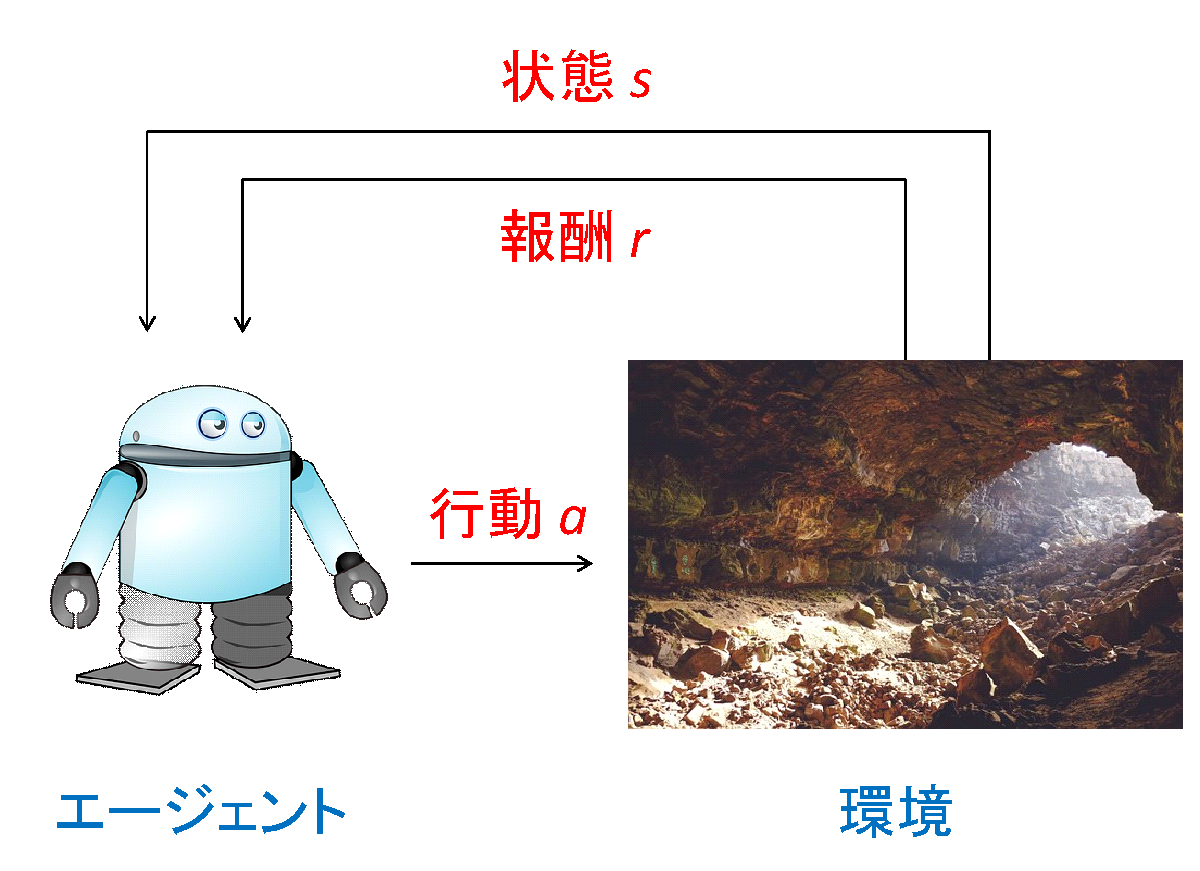
\includegraphics[width=80mm]{images/TsuruokaLab/rl.eps}
 \end{center}
 \caption{強化学習}
 \label{fig:rl1}
\end{figure}

強化学習を考える上での基本的な枠組みであるマルコフ決定過程 (Markov decision process, MDP) 
について簡単に述べる.マルコフ決定過程とは,
\begin{itemize}
\item 状態 (state) の有限集合 $S$
\item 行動 (action) の有限集合 $A$
\item 状態遷移関数 $P(s'|s,a)$: 状態$s \in S$ において行動$a \in A$をとった場合に状態$s' \in S$ に遷移する確率
\item 報酬関数 $R(s,a,s')$: 状態$s$から行動 $a$ によって状態$s'$ に遷移したときに得られる報酬
\end{itemize}
\noindent
によって構成され,エージェントの環境 (environment) を規定する.

いま,図\ref{fig:rl1} に示すように,この環境の中で,時刻 $t$ において状態 $s_t$ にあるエージェントが,行動 $a_t$ を選択したとする.
その結果,状態は $s_{t+1}$ に変化し,同時にエージェントは報酬 $r_{t+1}$ を受け取る.
強化学習におけるエージェントの目的は,現在から未来にわたる累積報酬

\begin{equation}
g_t = r_{t+1} + \gamma r_{t+2} + \gamma^2 r_{t+3} + \ldots = \sum_{k=0}^{\infty} \gamma^k r_{t+k+1}
\end{equation}

\noindent
を最大化する行動を選択することだと定式化される.$\gamma$ は割引率 (discount factor) 
と呼ばれる値であり,現時点ですぐに
もらえる報酬を未来の報酬よりもどれだけ重視するかを決めるパラメータである.

\section{Q学習}

強化学習のためのアルゴリズムとして最もよく知られているもののひとつに,Q学習 (Q-learning) と呼ばれる
アルゴリズムがある.いま,状態 $s$ のときに行動 $a$ を取り,その後,最善の行動を取り続けた場合に
得られる累積報酬の期待値を $Q^*(s,a)$ と書くものとする.$Q^*(s,a)$ は,Bellman 方程式と呼ばれる
以下の再帰的な関係式を満たす.
\begin{equation}
Q^*(s,a) = \sum_{s'} P(s'| s, a) (R(s, a, s') + \gamma \max_{a'} Q^*(s', a') )
\end{equation}

もし,任意の $s$ と $a$ の組み合わせに対して  $Q^*(s,a)$ がわかっているのであれば,
状態$s_t$において,エージェントは, $Q^*(s_t, a_t)$ が最大の行動 $a_t$ を選択すれば
累積報酬を最大化することができる.つまり,エージェントの行動選択の問題が解けたことになる.

もちろん通常は $Q^*(s,a)$ は未知なので,何らかの方法で推定する必要がある.
Q学習では,エージェントが環境のなかで行動するたびに,以下の更新式にしたがって
 $Q^*(s,a)$ の推定値である $Q(s,a)$ を更新する.
\begin{equation}
Q(s_t, a_t) \leftarrow Q(s_t, a_t) + \alpha [ r_{t+1} + \gamma \max_a Q(s_{t+1},a) - Q(s_t, a_t) ]
\end{equation}

%この更新式は次のように書かれることもある.
%
%\begin{equation}
%Q(s_t, a_t) \leftarrow (1 - \alpha) Q(s_t, a_t) + \alpha [ r_{t+1} + \gamma \max_a Q(s_{t+1},a) ]
%\end{equation}
%
%いずれにせよ,$Q(s_t, a_t)$ を

すなわち,$Q(s_t, a_t)$ を
\begin{equation}
r_{t+1} + \gamma \max_a Q(s_{t+1},a)
\end{equation}

\noindent
に近づけるように更新する.ただし,$\alpha \in [0,1]$ は学習率と呼ばれるパラメータである.Q学習では,
エージェントが全ての状態をゼロ以上の確率で訪れるように行動する場合,
学習率を徐々に下げていくことにより,$Q(s,a)$ が $Q^*(s,a)$ に収束することが知られている.


\begin{figure}[t]
 \begin{center}
  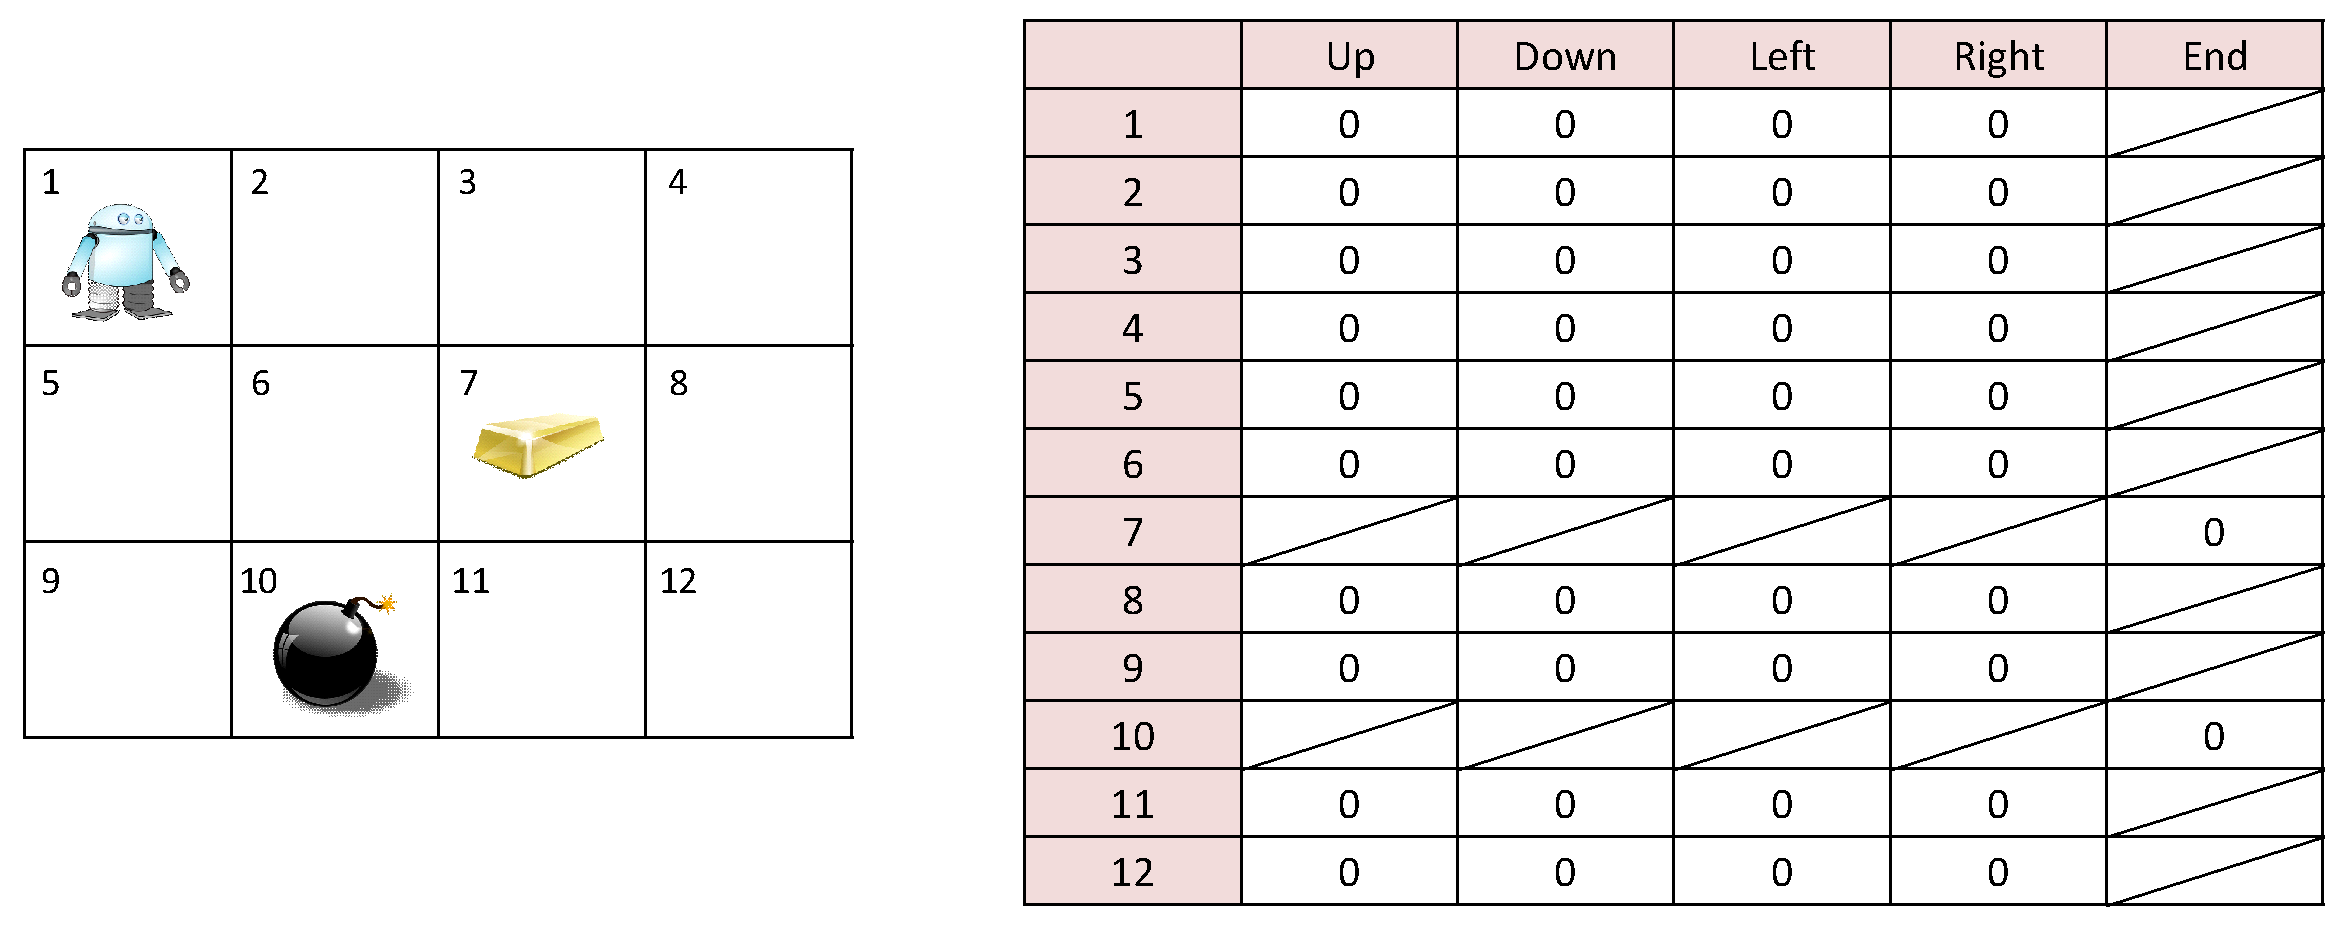
\includegraphics[width=140mm]{images/TsuruokaLab/ql1.eps}
 \end{center}
 \caption{Q学習(初期状態)}
 \label{fig:ql1}
\end{figure}

\subsection{テーブルを用いたQ学習の例}

Q学習の様子を例を用いて説明しよう.この例では,学習率$\alpha$は常に$1.0$,割引率$\gamma$ は $0.9$ 
であるとする.

図\ref{fig:ql1}に学習の初期状態を示す.エージェントは状態1から出発するものとする.
また,エージェントは各状態において Up, Down, Left, Right の4つの行動をとることができる.
ただし,状態7と状態10では,End という行動しかとることができず,それぞれ
$100$もしくは$-100$の報酬を受け取ったのち,エピソードが終了する.図の右側に示すテーブルは,
$Q(s,a)$ を表し,すべてゼロで初期化されている.

この状態からエージェントがランダムに行動した結果,状態7に到達したとする.すると,次のステップでは
行動として End をとり,報酬100を受け取り,エピソードが終了するため,更新式
\begin{equation}
Q(7, \mbox{End}) \leftarrow Q(7, \mbox{End}) + 1.0 \times [ 100 + 0.9 \times 0 - 0 ]
\end{equation}

\noindent
によって,$Q(7, \mbox{End})$ の値が 100 に更新される.次のエピソードで,状態10に到達した場合,
報酬として $-100$ を受け取るため,同様の計算により $Q(10, \mbox{End})$ の値は $-100$ となる.
この時点での$Q(s,a)$の値を格納するテーブルの状態を図\ref{fig:ql2}に示す.


\begin{figure}[t]
 \begin{center}
  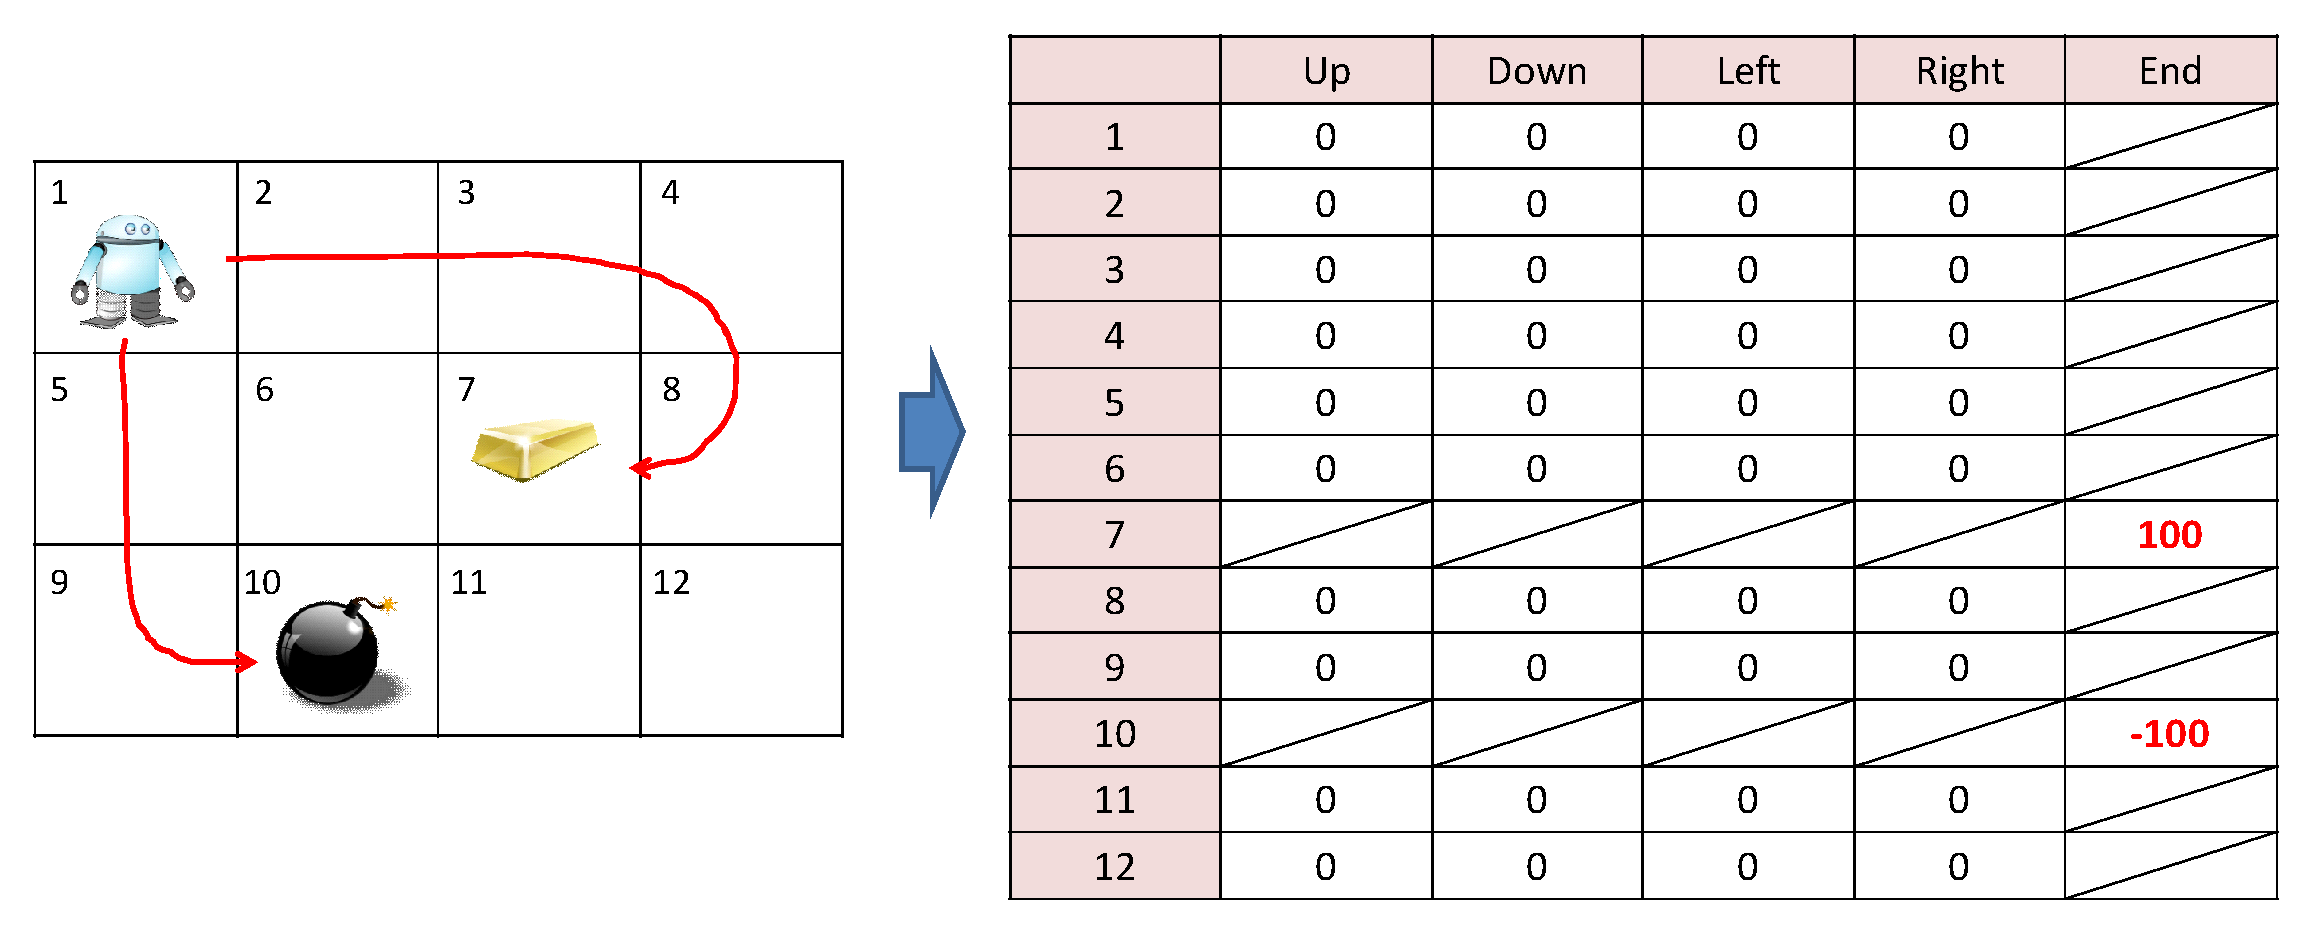
\includegraphics[width=140mm]{images/TsuruokaLab/ql2.eps}
 \end{center}
 \caption{Q学習(状態7と状態10を経験した後)}
 \label{fig:ql2}
\end{figure}

その後,エージェントは図\ref{fig:ql3} に示すように,状態3を経由して状態7に到達したとする.
この場合,更新式は,
\begin{equation}
Q(3, \mbox{Down}) \leftarrow Q(3, \mbox{Down}) + 1.0 \times [ 0 + 0.9 \times 100 - 0 ]
\end{equation}
\noindent
となるため,$Q(3, \mbox{Down}) $ の値が 90 に更新されることになる.


\begin{figure}[t]
 \begin{center}
  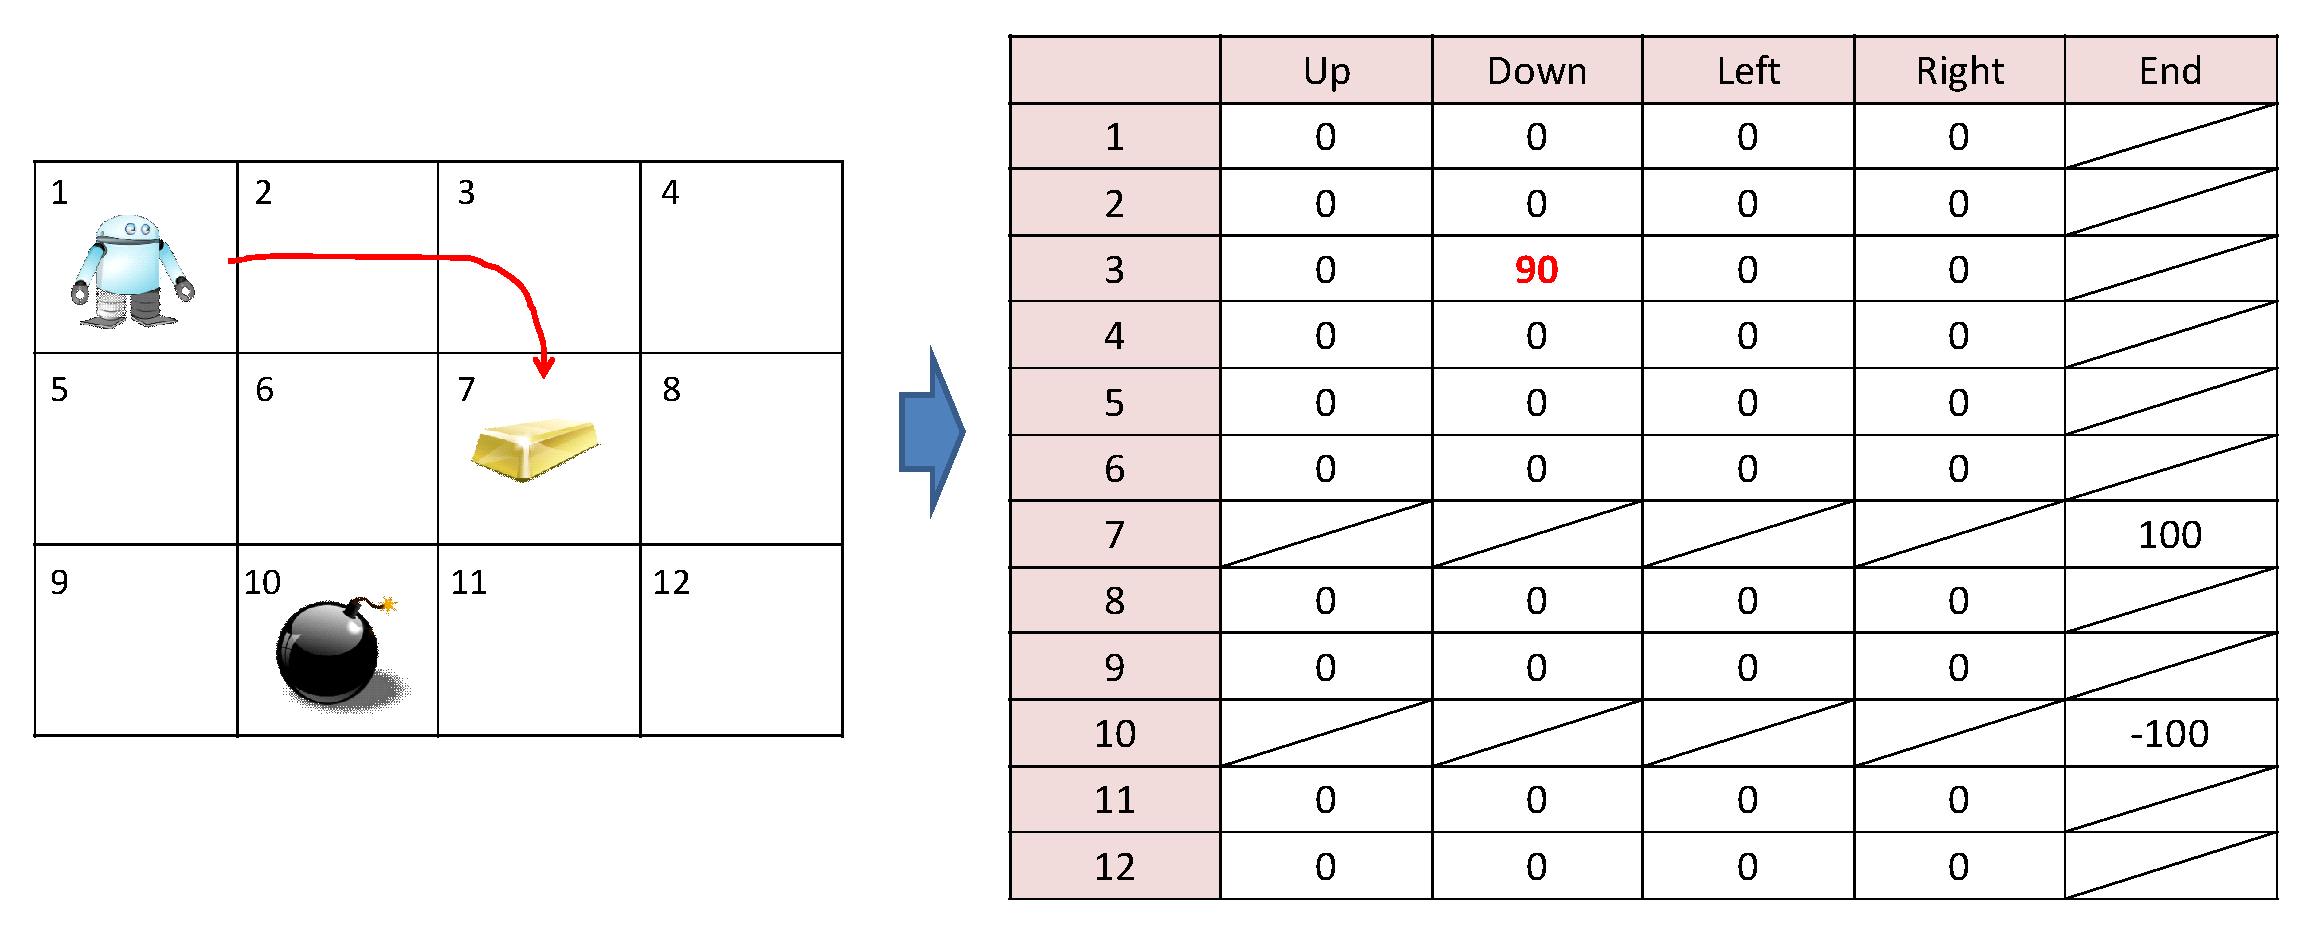
\includegraphics[width=140mm]{images/TsuruokaLab/ql3.eps}
 \end{center}
 \caption{Q学習(状態3から状態7に遷移した後)}
 \label{fig:ql3}
\end{figure}


\section{関数近似によるQ学習}

前節で説明したQ学習では,$Q(s,a)$の値を格納するためにテーブル(配列)を利用した.状態の数が
少ない場合にはこのような方法で学習を行うことができるが,現実の問題に強化学習を適用しようと
する場合,テーブルを利用したQ学習は不可能な場合が多い.例えば,ビデオゲームの AI を強化学習
で作ることを考えてみよう.入力として,ビデオゲームの画面,すなわち多数のピクセルから構成される画
像の情報を考えた場合,それによって決まる「状態」は無数に存在することになる.状態の数が非常に
大きい場合,テーブルに必要なメモリが莫大になることもさることながら,そもそもエージェントが同じ状態
を経験すること自体がまれになるため,学習が実質的にほとんど進まない.

関数近似 (function approximation) によるアプローチでは,$Q(s,a)$ をテーブルで表現するのではなく,
ニューラルネットワーク等,
パラメータ $\boldsymbol{\theta}$ によって規定される関数 $Q(s,a; \boldsymbol{\theta})$ で表現し,$Q^*(s,a)$ を精度
よく近似することを目指す.

いま,ある時点 $i$ でのパラメータを $\boldsymbol{\theta}_i$ としたとき,それをより適切
な値にするにはどのように更新すればよいだろうか? テーブルを用いたQ学習では,
$Q(s_t, a_t)$ を $r_{t+1} + \gamma \max_a Q(s_{t+1},a)$ に近づけるように更新を行ったのであった.
関数近似でも,それと同様の考え方により, $Q(s,a; \boldsymbol{\theta})$ を近づける目標として,
パラメータ $\boldsymbol{\theta}_{i-1}$ から計算される
\begin{equation}
y_i = r + \gamma \max_{a'} Q(s', a'; \boldsymbol{\theta}_{i-1})
\end{equation}
 を考え,それに対する
誤差が小さくするように更新を行うという方法が考えられる.誤差の基準として
2乗誤差を用いた場合は, 
\begin{equation}
L(\boldsymbol{\theta}_i) =  \mathbb{E}[ (y_i - Q(s,a; \boldsymbol{\theta}_i))^2 ]
\end{equation}
を最小化するようにパラメータを最適化する問題だとして解くことができる.

%関数近似に非線形関数であるニューラルネットワークを用いた手法として,Deep Q-Network 
%\cite{mnih2015humanlevel} がよく知られている.


